\PassOptionsToPackage{table,xcdraw}{xcolor}
\documentclass{beamer}

\definecolor{mybg}{RGB}{0,102,51}
\definecolor{emcolor}{RGB}{0,0,255}

\mode<presentation>
{
  \usetheme{Frankfurt}      % or try Darmstadt, Madrid, Warsaw, ...
  \usecolortheme{default} % or try albatross, beaver, crane, ...
  \usefonttheme{default}  % or try serif, structurebold, ...
  \setbeamertemplate{navigation symbols}{}
  \setbeamertemplate{caption}[numbered]
  \setbeamertemplate{footline}[frame number]
} 

% beamer stuff
%\useoutertheme[subsection=false]{smoothbars}
%\useinnertheme[shadow=true]{rounded}
%\usecolortheme{seagull}
%\setbeamerfont{block title}{size={}}
%\usefonttheme[onlylarge]{structurebold}
%\setbeamerfont*{frametitle}{size=\normalsize,series=\bfseries}
%\setbeamertemplate{navigation symbols}{}
%\setbeamercolor*{normal text}{fg=white,bg=gray}
%\setbeamercolor*{alerted text}{fg=white}
%\setbeamercolor*{example text}{fg=white}
%\setbeamercolor*{structure}{fg=white}
\AtBeginSection[]
{
  \begin{frame}%<beamer>
    \frametitle{Content}
    \tableofcontents[currentsection,currentsubsection,hideothersubsections]
  \end{frame}
}
% packages
\usepackage{enumerate}
\usepackage[table,xcdraw]{xcolor}
\usepackage{amssymb}
\usepackage{multicol}
\usepackage[normalem]{ulem}
\usepackage{wasysym}
\usepackage{listings}
\lstset{ %
  language=prolog,
%  frame=l,                   			% adds a frame around the code
  basicstyle=\scriptsize\ttfamily,	% use courier
  breaklines=false,
  xleftmargin=0em,
  aboveskip=0.5em,
  belowskip=0.5em,
%  belowcaptionskip=5em,
  numbers=left,
  backgroundcolor=\color{lightgray},
  frame=single,
  framerule=0pt
}
\usepackage{multimedia}
\usepackage{multirow}

% tikz stuff
\usepackage{tikz}
\usetikzlibrary{shadows}
\usetikzlibrary{shapes}
\usetikzlibrary{arrows}
\usetikzlibrary{calc}
\usetikzlibrary{fit}
\usetikzlibrary{backgrounds}
\usetikzlibrary{positioning}
\usetikzlibrary{chains}
\usetikzlibrary{scopes}
\usetikzlibrary{decorations}
\usetikzlibrary{decorations.text}
\usetikzlibrary{decorations.pathmorphing}
\usepackage{animate}

\usepackage{amsmath}
% \usepackage{paralist}

\newcommand{\myemph}[1]{{\bf {\color{emcolor}{#1}}}}

\begin{document}

\title{CLEMI}
\subtitle{CLustering to Evaluate Multiple Imputation}
\author{\myemph{Anthony Chapman} \\ \and Dr Steve Turner \and Dr Wei Pang \and Dr Lorna Aucott}
% \author[S.\,Cauvin \& D.\,Sleeman \& W. \,Vasconcelos]
% {%
%   \texorpdfstring{
%       \begin{columns}%[onlytextwidth]
%           \column{.38\linewidth}
%           \centering
%           \myemph{Samuel Cauvin}\\
%           \href{mailto:s.cauvin@abdn.ac.uk}{s.cauvin@abdn.ac.uk}
%           \column{.2\linewidth}
%           \centering
%           Derek Sleeman\\
%           \href{mailto:d.sleeman@abdn.ac.uk}{d.sleeman@abdn.ac.uk}
%           \column{.38\linewidth}
%           \centering
%           Wamberto Vasconcelos\\
%           \href{mailto:w.w.vasconcelos@abdn.ac.uk}{w.w.vasconcelos@abdn.ac.uk}
%       \end{columns}
%   }
%   {Samuel Cauvin \& Derek Sleeman \& Wamberto Vasconcelos}
% }`'
\institute{
Dept. of Applied Medical Sciences, University of Aberdeen \\Dept. of Computing Science, University of Aberdeen \\e-mail: \href{mailto:r01ac14@abdn.ac.uk}{r01ac14@abdn.ac.uk}
}

\date{
\includegraphics[height=1cm]{logo}\hfill
\includegraphics[height=1cm]{logo-farr}}
% \logo{
\includegraphics[height=1cm]{logo}\vspace{205pt}} % logo on ever slide
\maketitle

\begin{frame}
  \frametitle{Outline}
  \tableofcontents
\end{frame}

\section{Introduction}
\subsection{}

\begin{frame}
  \frametitle{Introduction}
  Motivation:
  \begin{itemize}
    \item Routinely acquired data has large amounts of missing data
    \item Most researchers carry out complete case analyses
    \item Need to use as much of the available data as possible. 
    \item Need something every researcher can trust
    \item A way to evaluate imputation
    \item Must be user friendly to most researchers (no need for a computing degree)
  \end{itemize}
\end{frame}

\begin{frame}
\frametitle{Missing Values in Raw Data}
\centerline{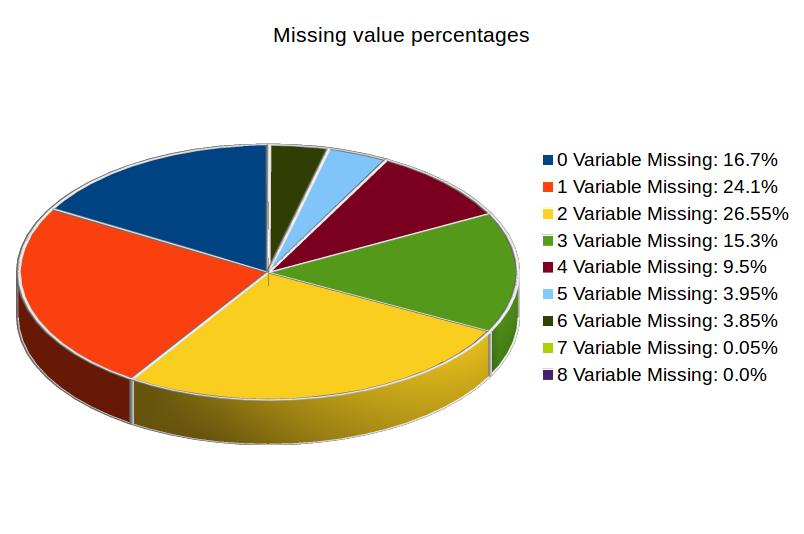
\includegraphics[width=\paperwidth]{missing-perc-equal}}
\end{frame}

% \begin{frame}
% \frametitle{Missing Values in Raw Data}
% \centerline{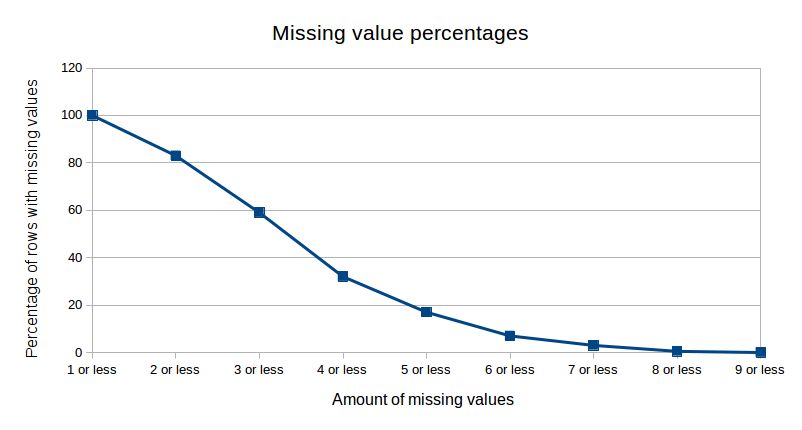
\includegraphics[width=\paperwidth]{missing-perc-min2}}
% \end{frame}

\begin{frame}
  \frametitle{Introduction}
  Motivation:
  \begin{itemize}
    \item Routinely acquired data has large amounts of missing data
    \item Most researchers carry out complete case analyses
    \item Need to use as much of the available data as possible. 
    \item Need something every researcher can trust
    \item A way to evaluate imputation
    \item Must be user friendly to most researchers (no need for a computing degree)
  \end{itemize}
\end{frame}

\begin{frame}
  \frametitle{Current Work}
  Imputation:
  \begin{itemize}
    \item Statistical Software (SPSS, R, StatSol)
    \item Mean Impuation, Multiple Imputation
    \item MICE: Multivariate Imputation by Chained Equations
  \end{itemize}
  Evaluation:
  \begin{itemize}
    \item No generalisation 
    \item Nothing
    \item Zilch
  \end{itemize}
\end{frame}

\section{Imputation}
\subsection{}

\begin{frame}
  \frametitle{Imputation - MICE}
  MICE - Multivariate Imputation by Chained Equations 
  \begin{itemize}
    \item Uses the whole dataset 
    \item Preserved the relations in the data
    \item Can work with longitudinal data 
  \end{itemize}
\end{frame}

\begin{frame}
  \frametitle{Imputation ctn.} 
  \centerline{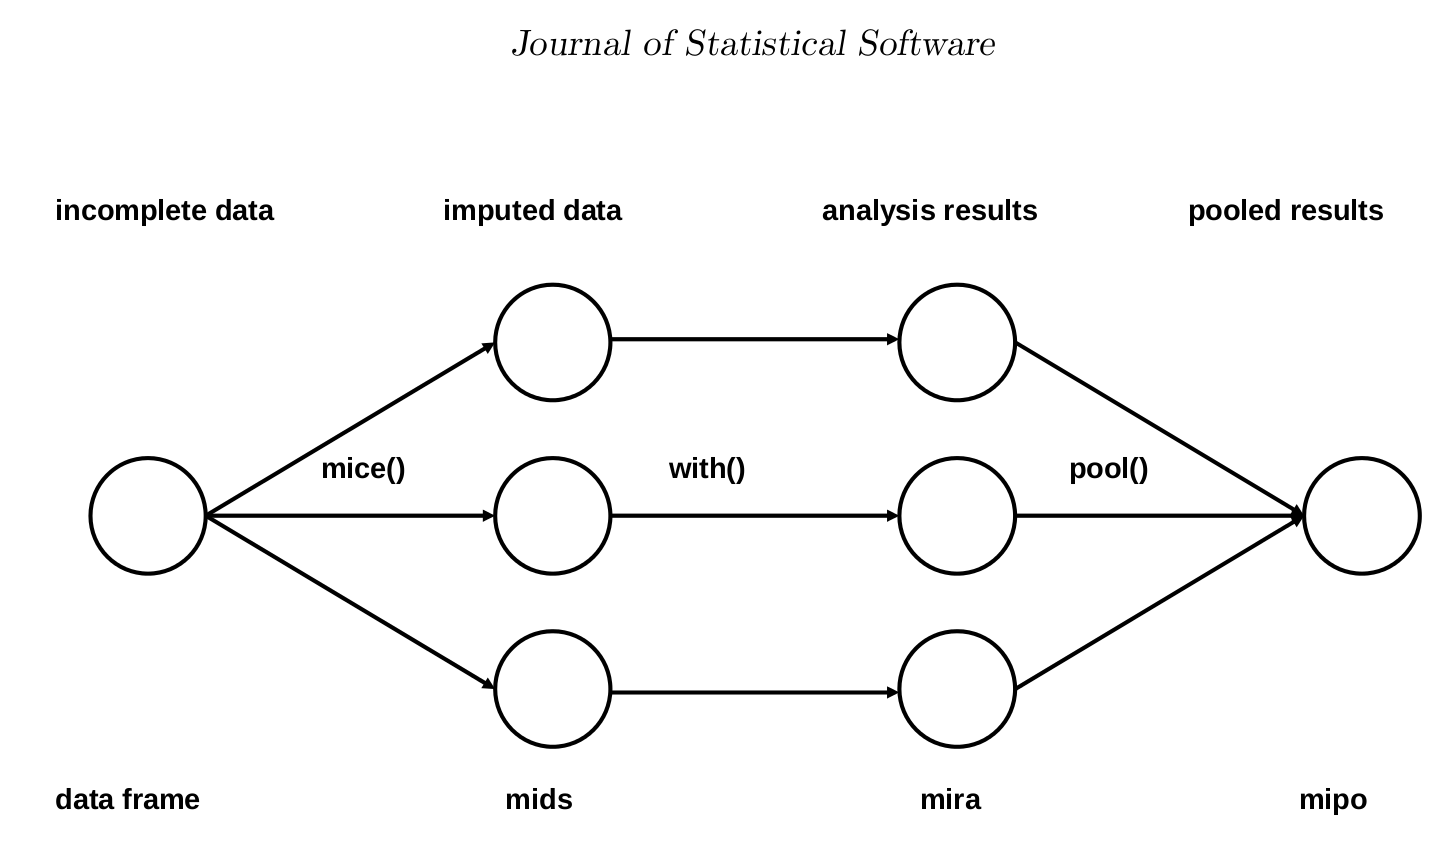
\includegraphics[width=\paperwidth]{mice}}
\end{frame}

\section{Benchmark}
\subsection{}

\begin{frame}
\frametitle{Benchmarks}
  % Why we need a benchmark:
  \begin{itemize}
    \item Needed to see effects of imputation
    \item Needed for a controlled test
    \item They are suppose to represent the truth
  \end{itemize}

\end{frame}

% \begin{frame}
% \frametitle{Benchmarks}
% Why we need a benchmark:
%   \begin{itemize}
%     \item Need something to compare against
%   \end{itemize}
% What a benchmark needs to be/do:
%   \begin{itemize}
%     \item Representative of the truth
%     \item Controlled testing
%   \end{itemize}
% \end{frame}

\begin{frame}
\frametitle{Benchmarks}
How to create a benchmark:
  \begin{itemize}
    \item Extract complete cases
    \item Analyse missingness in original dataset
    \item Create copies of the complete cases and apply missingness
    \item Every mini-me is a replica of the original   dataset but from the benchmark.
    % \item Apply missingness to multiple copies of the complete cases to create mini-mes 
  \end{itemize}
\end{frame}

\section{Evaluating Imputation}
\subsection{}

\begin{frame}
  \frametitle{Impute Artificially Incomplete Datasets}
  Apply MICE to all mini-me:
  \begin{itemize}
    \item Need to minimise uncertainty 
    \item Apply to multiple datasets
    \item Exact same method on all datasets
  \end{itemize}
\end{frame}

\begin{frame}
  \frametitle{Re-Cap}
  \centerline{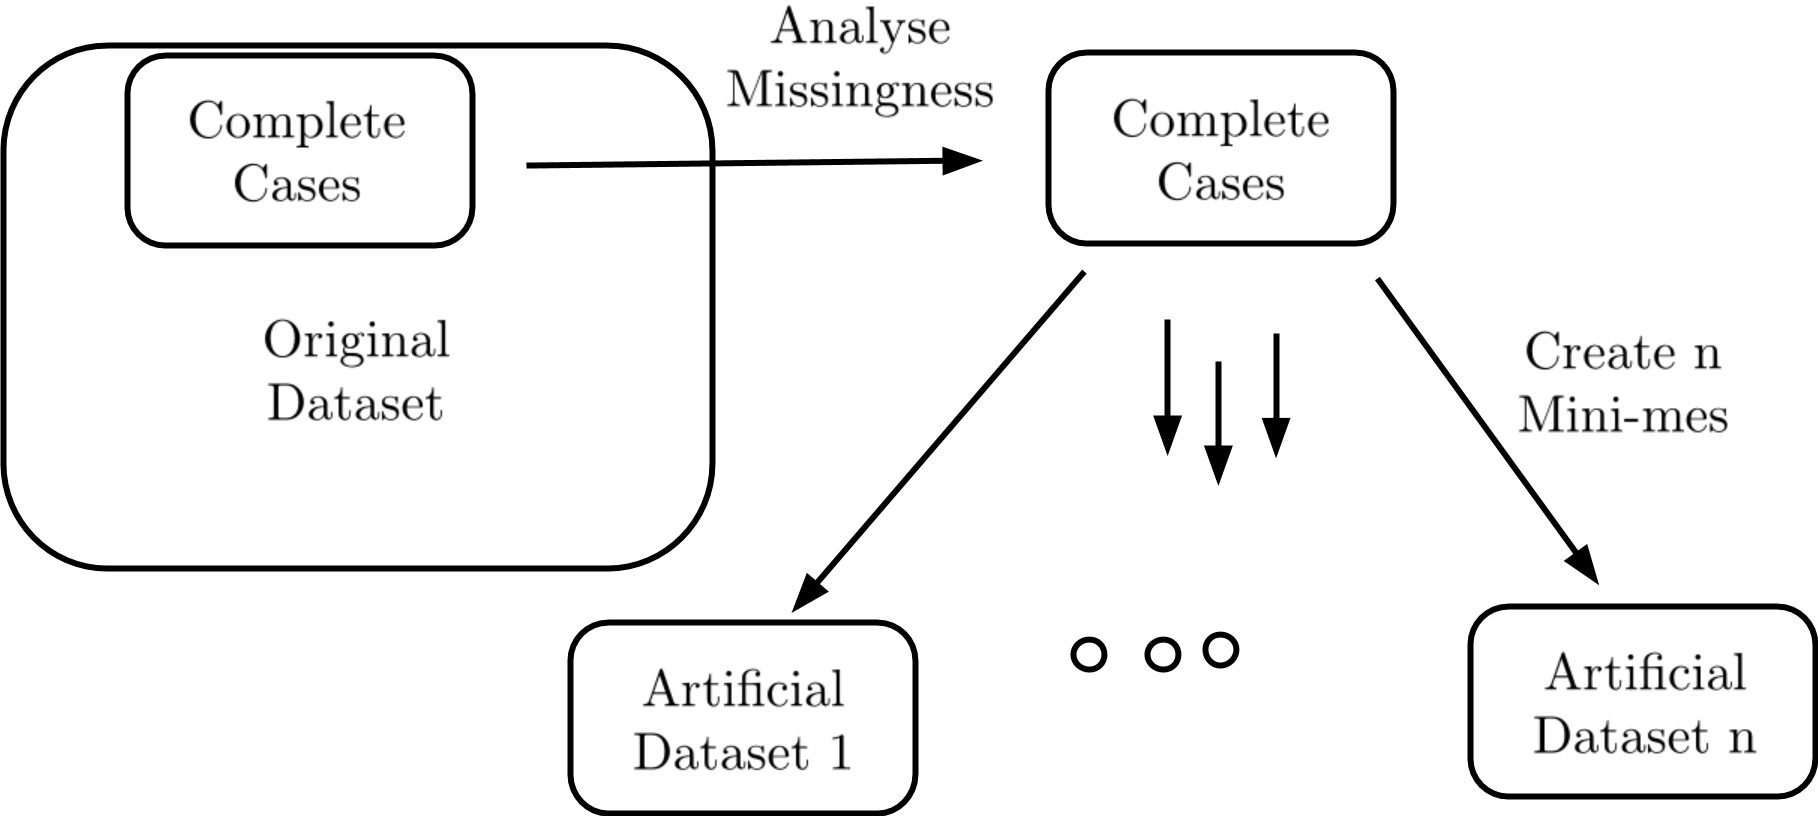
\includegraphics[width=\paperwidth]{datasets}}
  % picture of what datasets we have original, complete, mini-me, imputed mini-mes
\end{frame}

\begin{frame}
  \frametitle{Evaluation}
  Clustering:
  \begin{itemize}
    \item Group objects into a sets with similar objects
    \item Unsupervised 
    \item Good for higher dimensional data (Big Data) 
  \end{itemize}
\end{frame}

\begin{frame}
  \frametitle{Evaluation ctn.}
  % Distance Measure:
  % \begin{itemize}
  %   \item Clustering characteristics 
  %   \item 
  % \end{itemize}
  \centerline{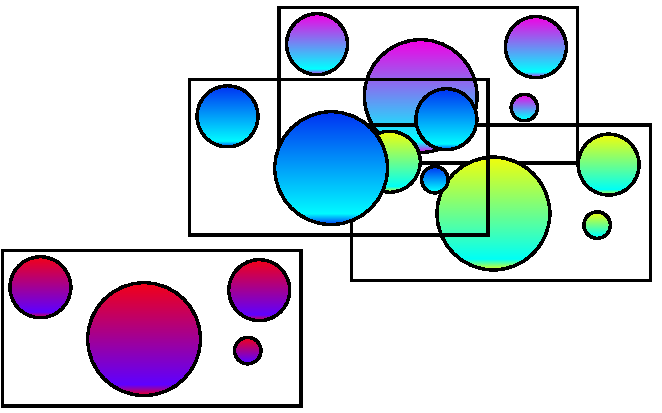
\includegraphics[width=\paperwidth]{clustering}}
\end{frame}

\begin{frame}
  \frametitle{Evaluation ctn.}
  Clustering:
  \begin{itemize}
    \item Get relevant clustering characteristics
    \item Compare imputed datasets to benchmark to see the effects
    \item Mean imputation as a reference
  \end{itemize}
\end{frame}

\section{Discussion}
\subsection{}

\begin{frame}
  \frametitle{Discussion \& Conclusion}
  Limitations
  \begin{itemize}
    \item Output is subjective 
    \item Some may over-interpret the results
    \item What if the complete subset is too small
  \end{itemize}
  Outcomes
  \begin{itemize}
    \item Optimised number of ignored records 
    \item Compare different imputation methods
    \item Optimize imputation features
  \end{itemize}
  To Consider
  \begin{itemize}
    \item Use a modelling to verify the outcome 
    \item Use any imputation method
  \end{itemize}
\end{frame}

%   \begin{frame}
%   \frametitle{Outcomes}
%   \begin{itemize}
%     \item Optimised number of ignored records 
%     \item Compare different imputation methods
%     \item Optimize imputation features
%   \end{itemize}
% \end{frame}

% \begin{frame}
%   \frametitle{Future Work}
%   Missing data analysis:
%   \begin{itemize}
%     \item Use a model to verify if it's true (if it works, the model must be similar)
%     \item Use any imputation method
%   \end{itemize}
% \end{frame}

\begin{frame}
\frametitle{Thanks \& Questions}
\centerline{\Huge \myemph{Thanks for your attention!}}
\centerline{\Huge \myemph{Question \& Comments }}
\end{frame}

\end{document}


